\documentclass{beamer}
\mode<presentation>
{
  \usetheme[headline]{ICL}
  % or ...

  \setbeamercovered{transparent}
  % or whatever (possibly just delete it)
}
%\setbeamertemplate{headline}[default]
%\setbeamercovered{transparent}
%\setbeamertemplate{footline}[default]
%\setbeamertemplate{headline}[split]
\usepackage[T1]{fontenc}
\usepackage[utf8]{inputenc}
\usepackage{times}
\usepackage[english]{babel}
\usepackage{color}  
\usepackage{pifont}
\usepackage{multicol}
\usepackage{multirow}
\usepackage{pgf}
\usepackage{graphicx}
\usepackage{hyperref}
%\usepackage{algorithm}
%\usepackage{algorithmic}
\usepackage{xspace}
\usepackage{transparent}

%%%%%%%%%definition des variables%%%%%%%%%%%%%%%
%\usepackage[latin1]{inputenc}
%\usepackage[T1]{fontenc}
%\usepackage{textcomp}
%\usepackage{lmodern}
%\usepackage{listings} 


%%%%%%%%%%%%%%%%%%%%%%%%%%%%%
\def\sujet{}
\def\projet{Enabling Partial Pivoting in Task Flow LU Factorization} 
\def\etape{}
\def\gA{Omar \textsc{Zenati}}
\def\gB{Supervisors: G. Bosilca, P. Ramet}

\definecolor{borange}{RGB}{248,170,78}

%%%%%%%%%%%%%%%% Header %%%%%%%%%%%%%%%%
 \title[Enabling Partial Pivoting in Task Flow LU Factorization]{
        {\bfseries \projet\\} 
        {\bfseries \huge \sujet}
        {\small Master Defense}
}


\titlegraphic{
  
\includegraphics[scale=0.5]{icl.png}
  \hfill
  
\includegraphics[scale=0.3]{inria.png}
  }
\date{September 13, 2012}

\author[Zenati]{
  {\normalsize \bfseries \sffamily} {\large \gA}\\
  \vspace{1cm}
  {\normalsize \bfseries \sffamily} {\large \gB}\\
}


\AtBeginSection[]{
  \begin{frame}{Summary}
  \tableofcontents[currentsection,subsectionstyle=shaded]
  \end{frame}
}

\AtBeginSubsection[]{
  \begin{frame}{Summary}
  \tableofcontents[currentsection,currentsubsection]
  \end{frame}
}
\begin{document}

\begin{frame}
\maketitle
\end{frame}

\begin{frame}
\begin{itemize}
\item Three months at \textit{Innovative Computer Laboratory}
\end{itemize}
\begin{center}

\includegraphics[width=0.6\textwidth]{icl-claxton.jpg}
\end{center}
\begin{itemize}
\item Three months at \textit{Inria Bordeaux Sud-Ouest}
\end{itemize}
\begin{center}
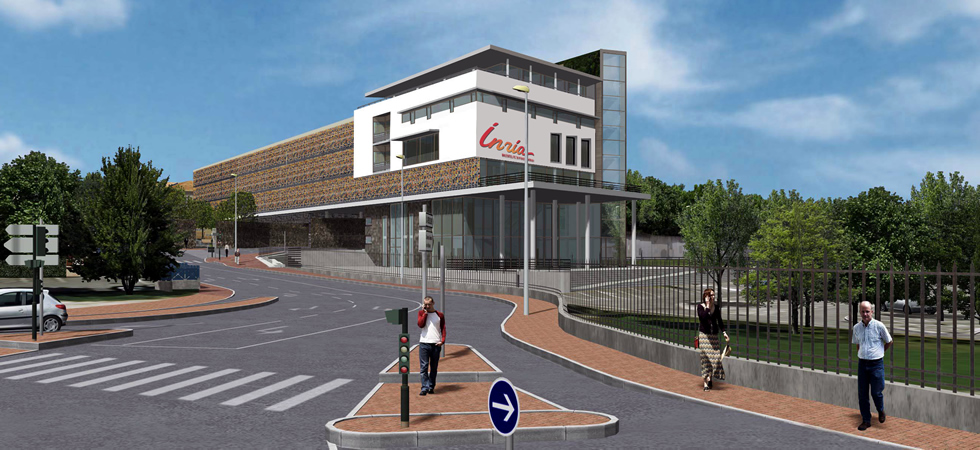
\includegraphics[width=0.5\textwidth]{bandeau-home-bordeaux.jpg}
\end{center}
\end{frame}

\begin{frame}{Summary}
\tableofcontents
\end{frame}

\section[Context]{Context and Motivations}
The work presented in this report was carried out under an internship. This was performed during 3 months in the Innovative Computer Laboratory (ICL) and 3 months in the Inria of Bordeaux. It is a part of the project \emph{Matrices Over Runtime Systems @ Exascale} (MORSE) which aim to design dense and sparse linear algebra methods that achieve the fastest possible time to an accurate solution on large-scale multi-core systems with GPU accelerators.

\subsection*{Innovative Computer Laboratory}
Attached to the university of Tennessee, the Innovative Computer Laboratory (ICL) is one of the world leader laboratory in the field of high performance computing (HPC). ICL was established by the Dr Jack Dongarra from 1989. Since its inception, ICL produced and participated to several applications of high value to the HPC community including: ATLAS, BLAS, LAPACK, MPI, Netlib, PAPI, ScaLAPACK, Top 500 \dots

Today, ICL continues in its desire to contribute to science. In this dynamic, I worked with the DPLASMA team where my mission was to apprehend the \dague runtime system first and then to study the feasibility of task flow LU decomposition over PTG using \dague as practical tool.

\subsection*{Inria}
Public science and technology institution established in 1967, Inria is is the only public research body fully dedicated to computational sciences. Combining computer sciences with mathematics, Inria’s 3,400 researchers strive to invent the digital technologies of the future.

I worked with the BACCHUS team which aim to develop and validate numerical methods adapted to physical problems. Firstly, my goal was to continue the work I started in ICL. Then, my mission was to take in hand the StarPU runtime system and implement its task flow LU decomposition in order to compare performances of PTG and sequential task flow.

\section[Without Pivoting]{LU Decomposition Without Pivoting ($A=LU$)}
\begin{frame}{Task flow LU ($A = LU$)}
In order to cope with the task flow model, linear algebra algorithms are expressed in terms of tasks operating on fine grain squares sub-matrices, also called tiles.
\begin{columns}
\begin{column}{0.02\textwidth}
\end{column}
\begin{column}{0.5\textwidth}
\begin{overprint}
\includegraphics<1>[width=0.9\linewidth]{free}
\includegraphics<2>[width=0.8\linewidth]{free_tiled}
\includegraphics<3>[width=0.8\linewidth]{task_getrf}
%\includegraphics<4>[width=0.8\linewidth]{task_trsm_l}
\includegraphics<4>[width=0.8\linewidth]{task_trsm_u}
\includegraphics<5>[width=0.8\linewidth]{task_gemm}
%\includegraphics<7>[width=\linewidth]{dag_getrf_sp}
\includegraphics<6>[scale=0.3]{step_lu}
\end{overprint}
\end{column}
\begin{column}{0.45\textwidth}
\begin{overprint}
\includegraphics<3>[width=0.8\linewidth]{getrf_getrf}
%\includegraphics<4>[width=0.8\linewidth]{getrf_trsm_l}
\includegraphics<4>[width=0.8\linewidth]{getrf_trsm_u}
\includegraphics<5>[width=0.8\linewidth]{getrf_gemm}
\includegraphics<6>[width=0.8\linewidth]{getrf}
\end{overprint}
\end{column}
\end{columns}
\begin{flushleft}
\onslide*<2>{Tiles are not contiguous in memory}
\onslide*<3>{Task to factorize diagonal tiles: GETRF}
\onslide*<4>{Task to update other panel tiles and block line tiles: TRSM\_L and TRSM\_U}
\onslide*<5>{Task to update trailing sub-matrix: GEMM}
\end{flushleft}
\end{frame}

%\begin{frame}{Task Flow LU}
%\framesubtitle{Example on matrix of 3*3 tiles}
%\begin{columns}
%\begin{column}{0.02\textwidth}
%\end{column}
%\begin{column}{0.3\textwidth}
%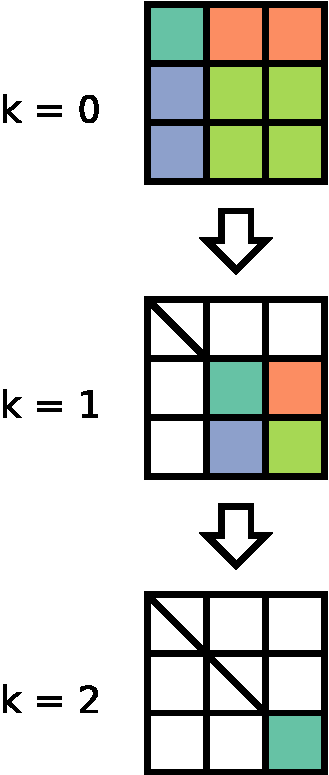
\includegraphics[scale=0.5]{step_lu}
%\end{column}
%\begin{column}{0.6\textwidth}
%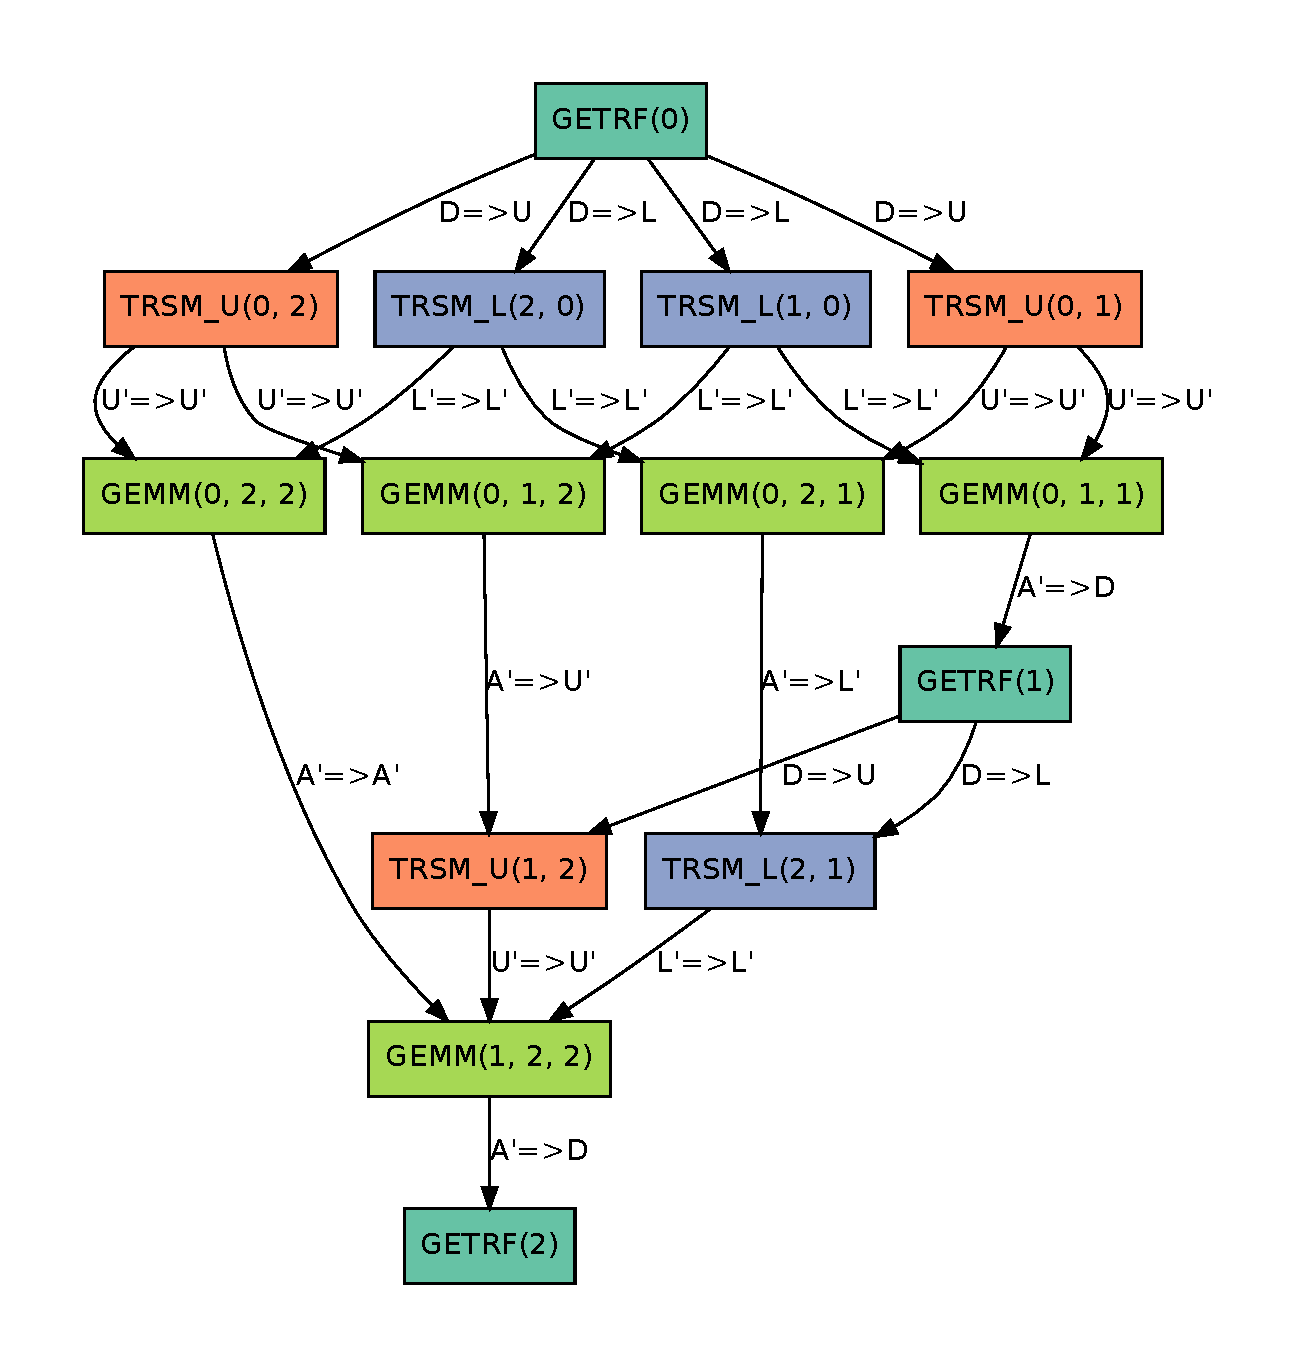
\includegraphics[width=\linewidth]{getrf}
%\end{column}
%\end{columns}
%\end{frame}

\section[Partial Pivoting]{LU Decomposition with Partial Pivoting ($PA=LU$)}
%\begin{frame}{LU decomposition problem}
%\begin{columns}[c]
%\begin{column}{0.02\textwidth}
%\end{column}
%\begin{column}{0.45\textwidth}
%\begin{tabbing}
%Let be $A$ a $n*n$ square matrix\\
%For \= $k$ from $1$ to $n$\\
%\>\visible<3->{\alert{Search for pivot then swap}}\\
%\> For \=$i$ from $k+1$ to $n$\\
%\>\> $a_{i,k} = a_{i,k}/a_{k,k}$\\
%\> For \=$i$ from $k+1$ to $n$\\
%\>\> For \=$j$ from $k+1$ to $n$\\
%\>\>\> $a_{i,j} = a_{i,j}-a_{i,k}*_{k,j}$\\
%\end{tabbing}
%\end{column}
%\begin{column}{0.02\textwidth}
%\end{column}
%\begin{column}{0.45\textwidth}
%\begin{itemize}
%\item $a_{k,k}$ may be close to zero
%\item Numerical value may be deteriorated due to fixed precision used by computers
%\end{itemize}
%\pause
%$\Rightarrow$ LU decomposition is not stable
%\end{column}
%\end{columns}
%\visible<3>{\alert{Solution is pivoting}}
%\end{frame}
%
%\begin{frame}{Partial Pivoting Algorithm}
%
%{
%The partial pivoting consist to look for the element with the maximal absolute value on the $k^{th}$ column from $a_{k,k}$, then swap its row with the row consisting $a_{k,k}$.
%}
%{
%The partial pivoting is:
%\begin{itemize}
%\item Practically stable and accurate
%\item Commonly used in the scientific community
%\item Used in the LINPACK benchmark to rank the TOP 500 super-computers
%\end{itemize}
%}
%\pause
%\begin{exampleblock}{Problem:}
%Complex to adapt to the task flow model
%\end{exampleblock}{}
%\end{frame}

%\subsection{Panel Factorization}

\begin{frame}{Panel Factorization Problems}
\framesubtitle{Tasks of panel factorization}
\begin{center}
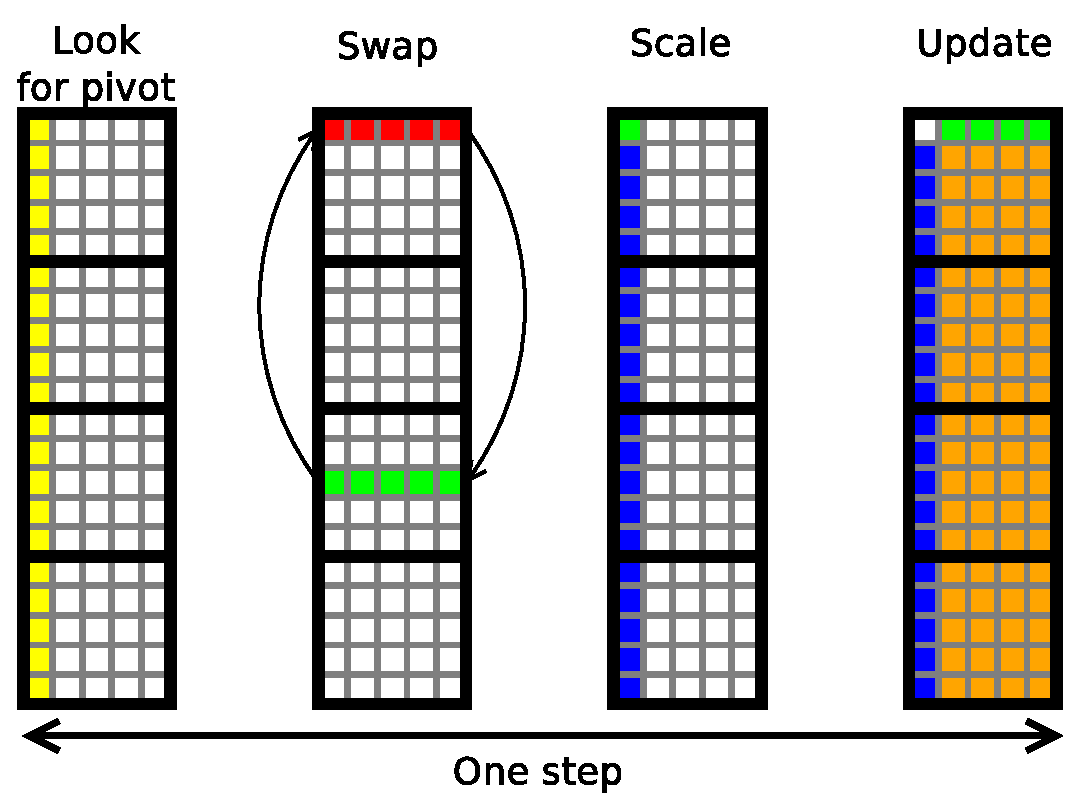
\includegraphics[width=0.6\textwidth]{panel_operation}
\end{center}
\begin{center}
\pause
\begin{itemize}
\item \alert{Look for a pivot is distributed over several tiles}
\item \alert{Tasks are fine grained}
\end{itemize}
\end{center}
\end{frame}

\begin{frame}{Panel Factorization Problems}
\framesubtitle{Reduce fine grained tasks}
\begin{center}
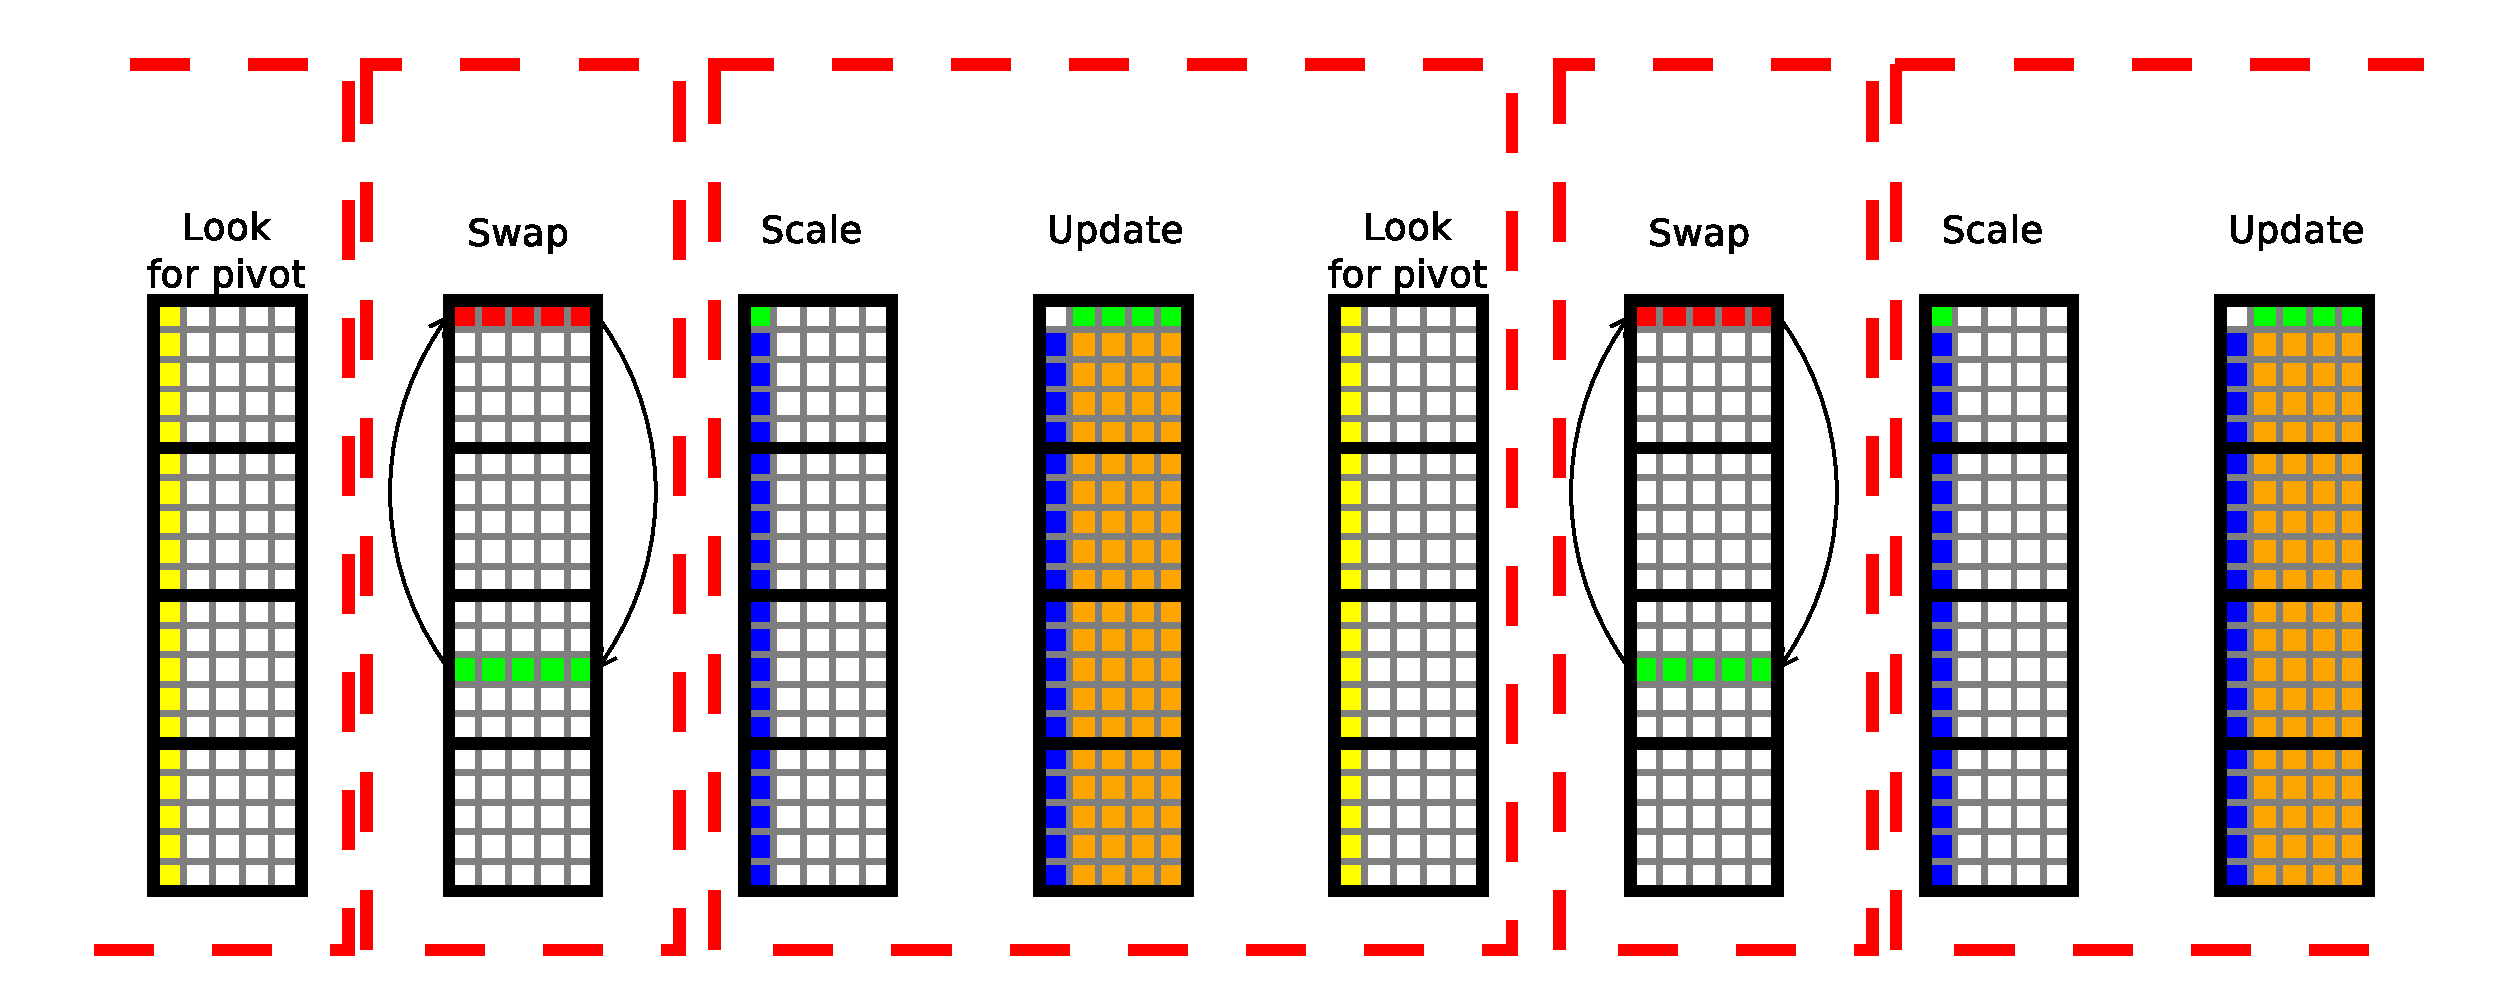
\includegraphics[width=0.8\textwidth]{merge}
\end{center}
\end{frame}


\begin{frame}{Panel Factorization Problems}
\framesubtitle{Natural task flow of panel factorization}
\begin{center}
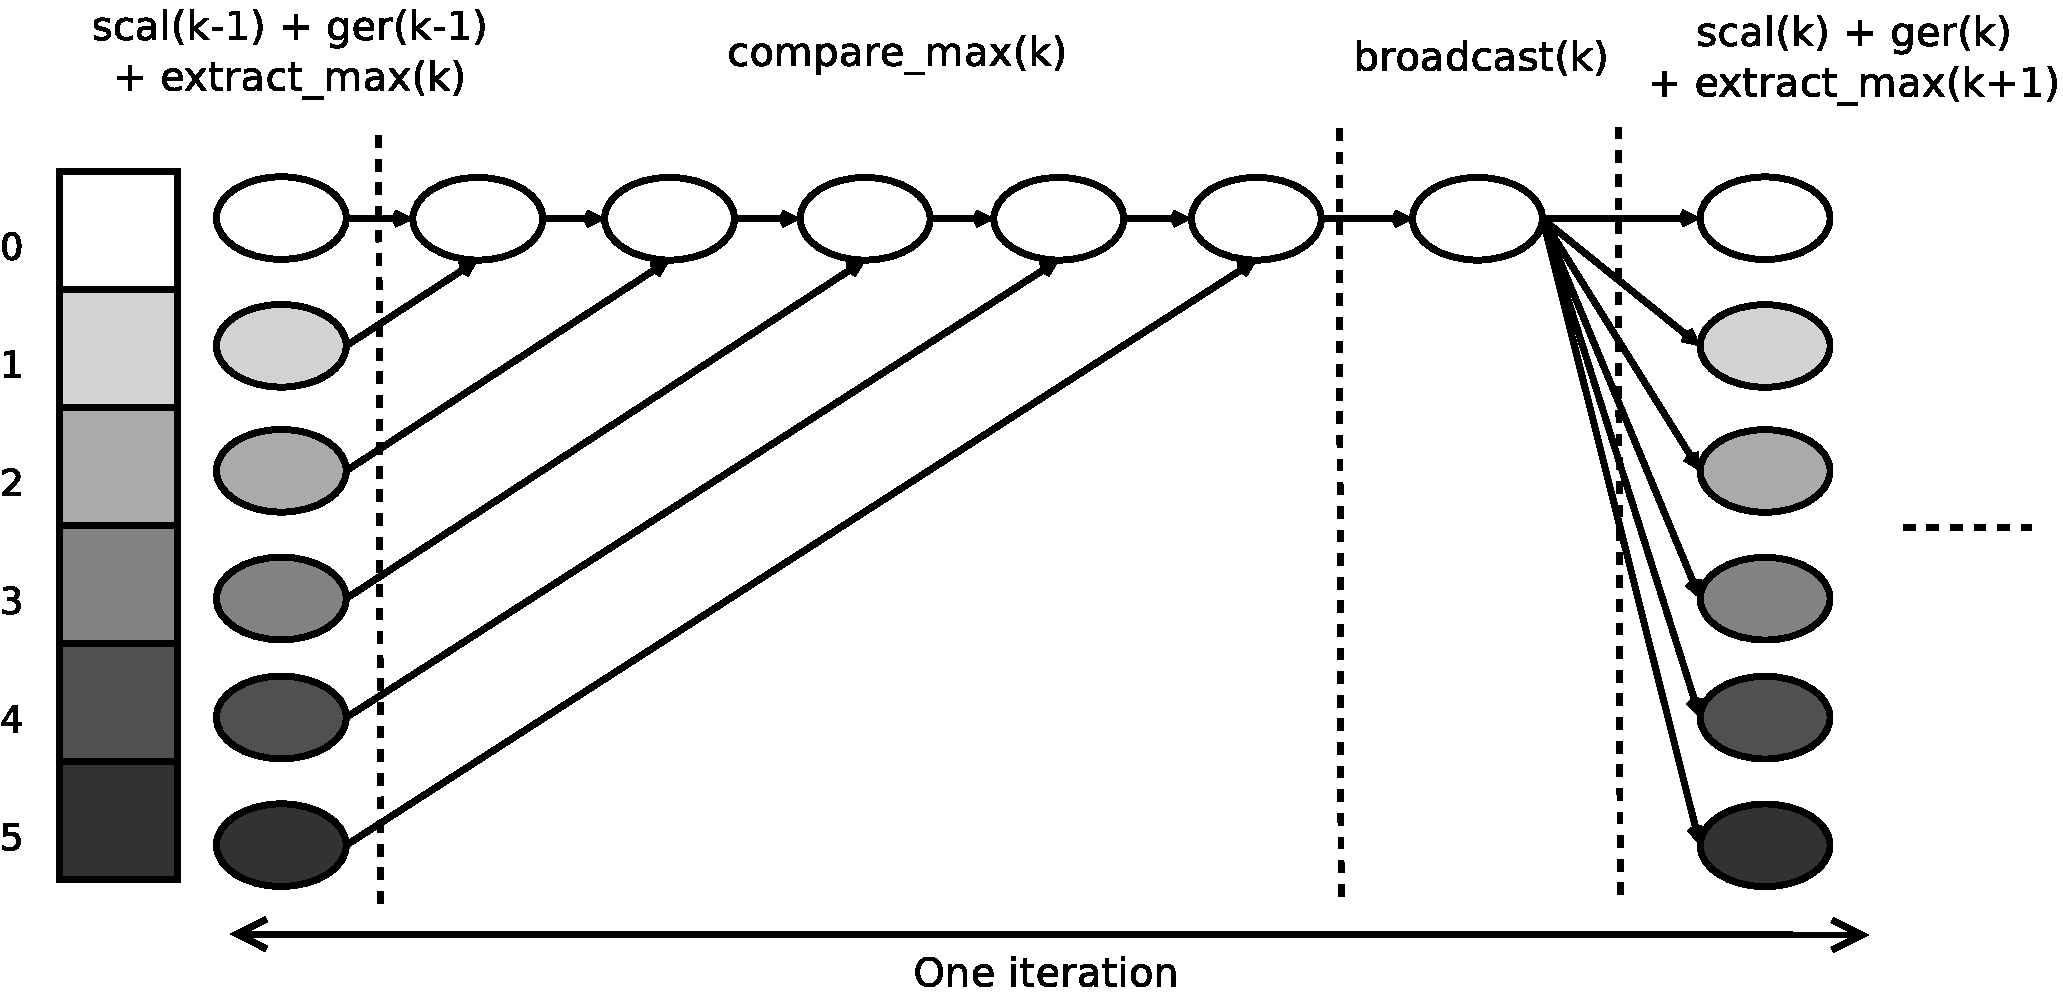
\includegraphics[width=0.6\textwidth]{natural_tf_bw}
\end{center}
\pause
\begin{center}
$\Rightarrow$ Serialized task flow!
\end{center}
\pause
\begin{exampleblock}{Optimizations:}
Use \emph{all\_reduce} operation (using Bruck's algorithm)
\end{exampleblock}{}
\end{frame}

\begin{frame}{Panel Factorization Problems}
\framesubtitle{Optimized task flow of panel factorization for distributed architectures}
\begin{center}
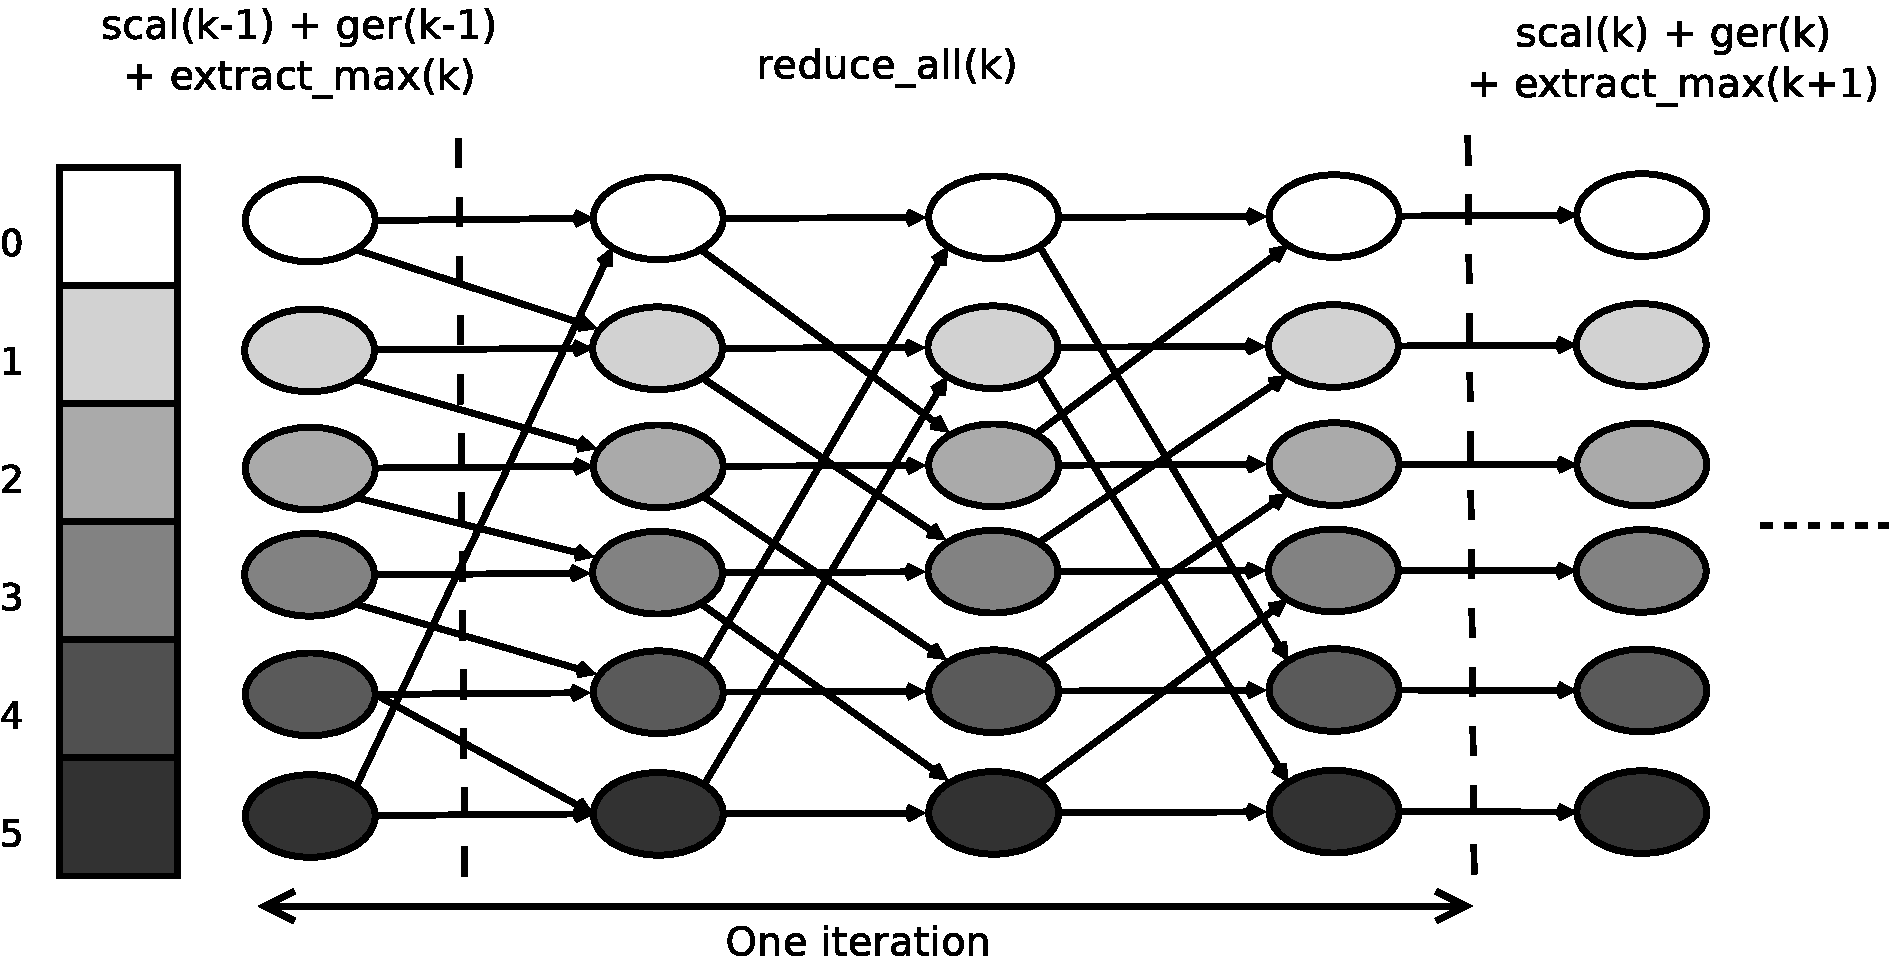
\includegraphics[width=0.6\textwidth]{distributed_tf_bw}
\end{center}
\end{frame}

\begin{frame}{Panel Factorization Problems}
\framesubtitle{Optimized task flow of panel factorization for hierarchical architectures}
\begin{center}
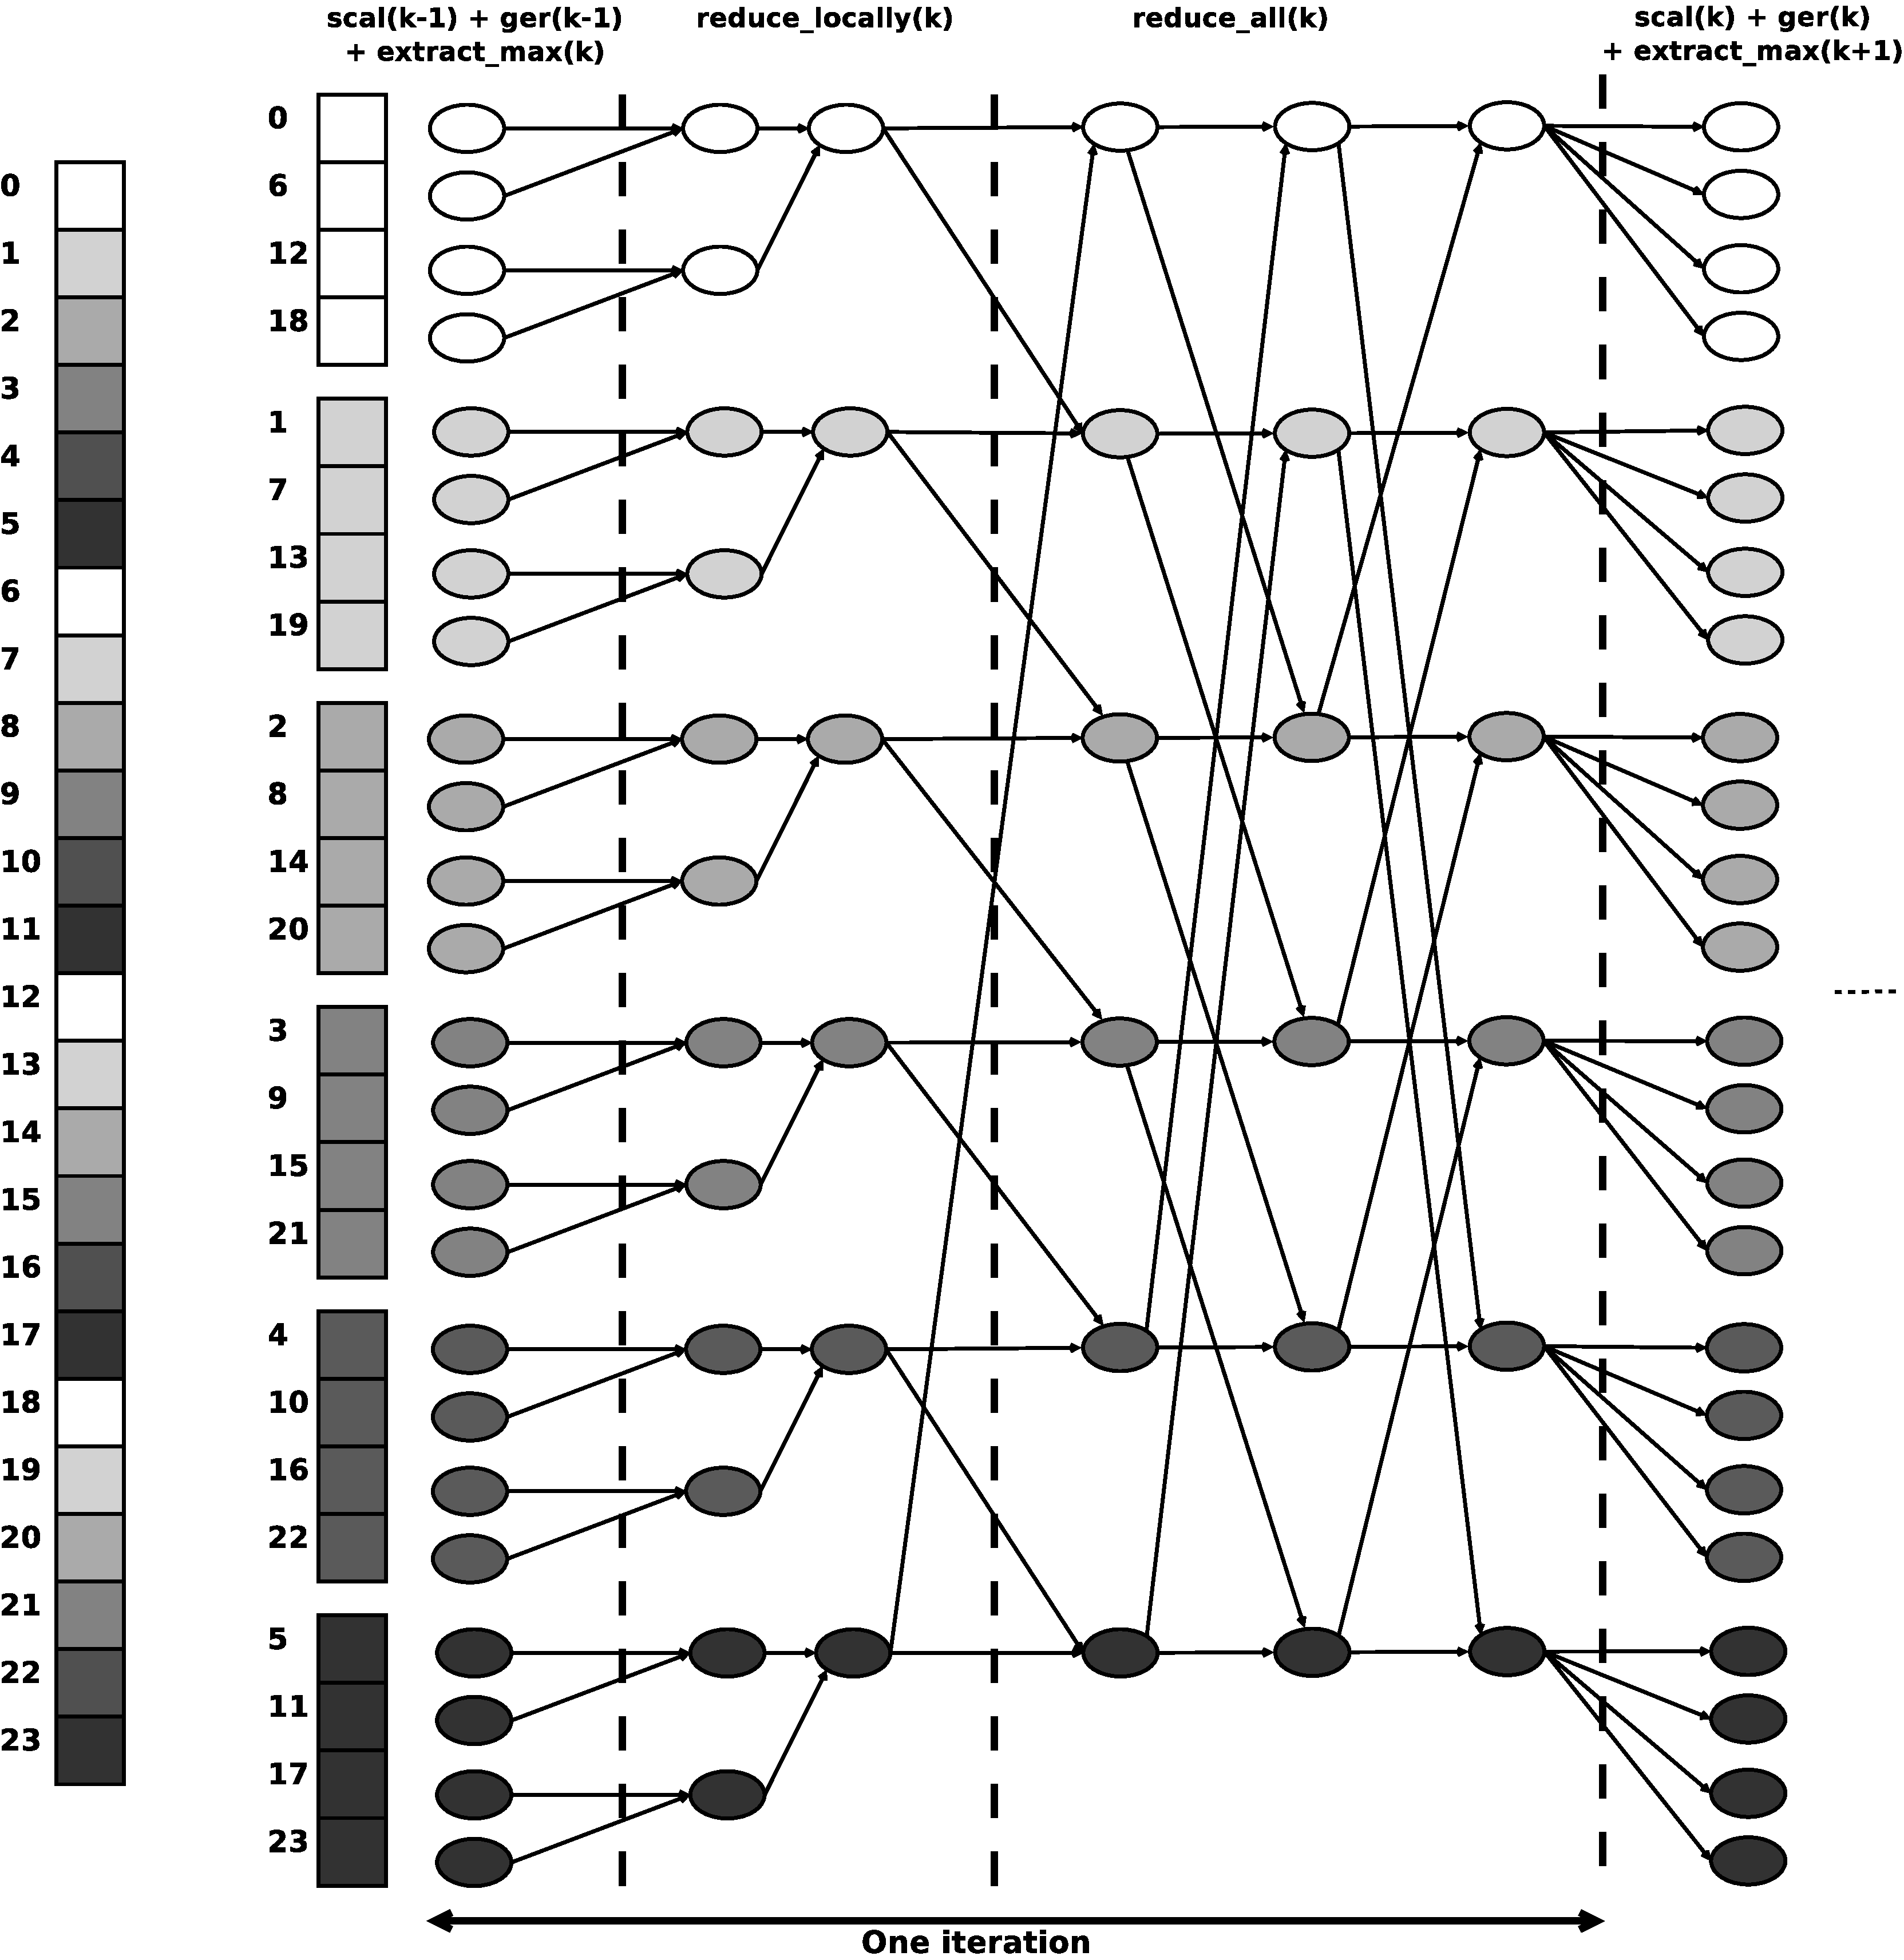
\includegraphics[width=0.55\textwidth]{hybrid_tf_bw}
\end{center}
\end{frame}

%\subsection{Update of Trailing Sub-matrix}

\begin{frame}{Update Problems}
\framesubtitle{Update trailing sub-matrix}
\begin{columns}
\begin{column}{.50\textwidth}
\begin{center}
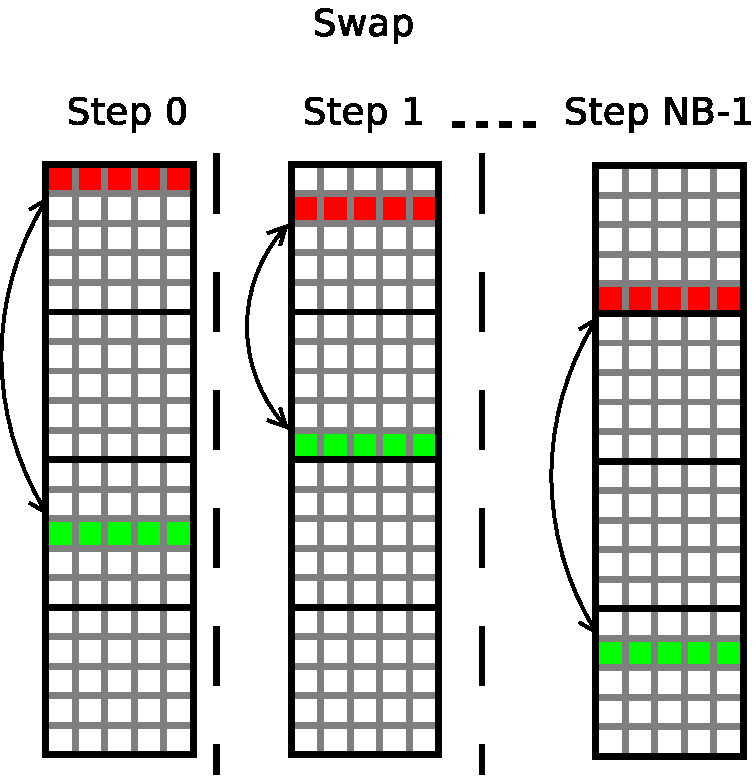
\includegraphics[scale=0.2]{update_swap.pdf}
\end{center}
\end{column}
\hfill
\begin{column}{.50\textwidth}
The upper tile exchange rows with other tile depending on pivots values.
\end{column}
\end{columns}
\pause
\begin{footnotesize}
\begin{exampleblock}{Problem \visible<3>{$\rightarrow$ Solutions}}
\begin{itemize}
\item Dynamic decision for a static DAG
\visible<3>{$\rightarrow$ Generate tasks for all possible communications?}
\item Pivots implies swaps in a specific order
\visible<3>{$\rightarrow$ Use permutation instead of pivots}
\item Serialized communications
\visible<3>{$\rightarrow$ Separate Swap from/into upper tile}
\end{itemize}
\end{exampleblock}{}
\end{footnotesize}
\end{frame}



\section{Performance}
\begin{frame}
\begin{center}
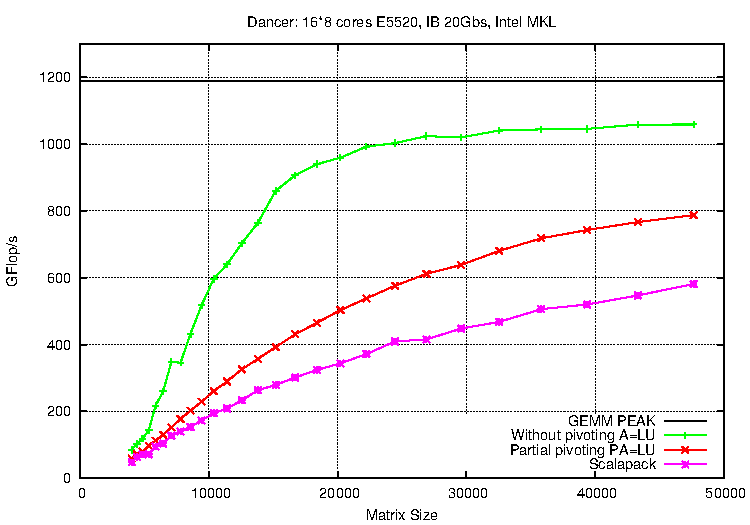
\includegraphics[width=0.8\textwidth]{gepp}
\end{center}
\end{frame}

\section*{Conclusion}
\begin{frame}{Conclusion and future work}
Conclusion :
\begin{itemize}
\item Implemented static pivoting ($A=LU$) on DAGuE and StarPU
\item Implemented partial pivoting ($PA=LU$) on DAGuE and StarPU
\item Exhibited the feasibility of partial pivoting on task flow model
\item Obtained encouraging performances with partial pivoting over DAGuE
\item Performances of partial pivoting over StarPU still not exploitable
\end{itemize}
Future work :
\begin{itemize}
\item Integrate GPU pivoting operations to DAGuE and StarPU
\item Try other startegies of panel factorizations on several methods
\item Build a new benchmark based on the DAGuE partial pivoting
\end{itemize}
\end{frame}

\begin{frame}
\begin{center}
\huge{Thank you !}
\end{center}
\end{frame}

\begin{frame}{ANNEXE}
\framesubtitle{Using permutations instead pivots}
\begin{columns}[c]
\begin{column}{0.02\textwidth}
\end{column}
\begin{column}{0.45\textwidth}
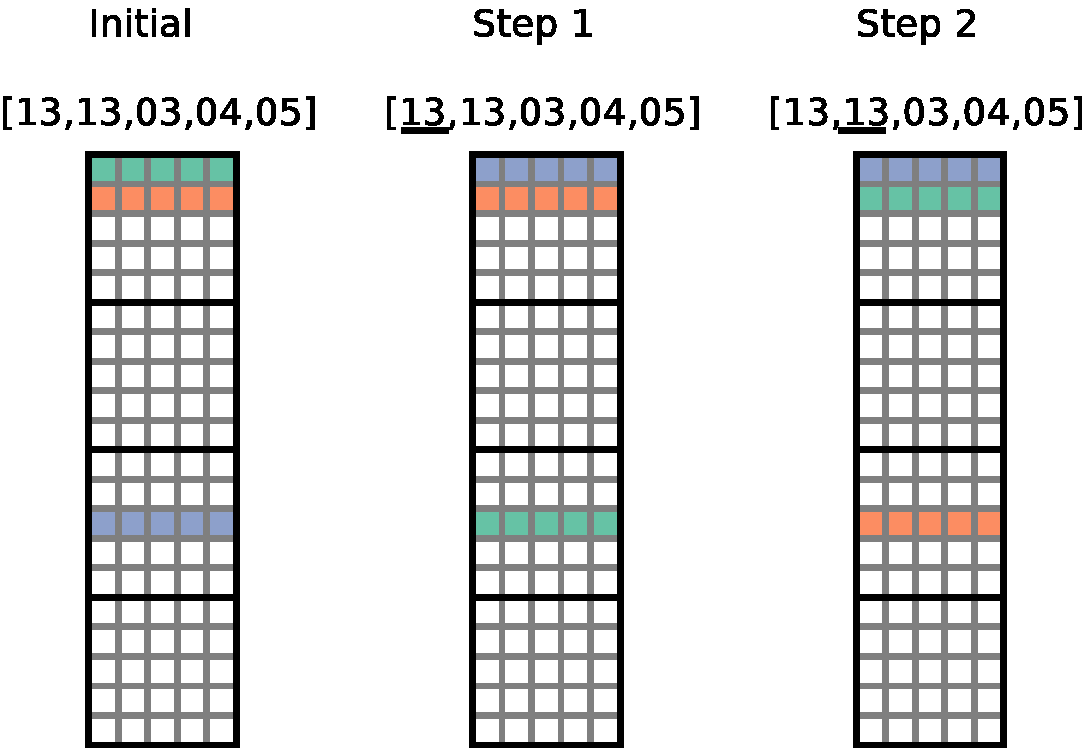
\includegraphics[width=\textwidth]{pivots_step}
\end{column}
\vline
\begin{column}{0.02\textwidth}
\end{column}
\begin{column}{0.45\textwidth}
\includegraphics<2>[width=\textwidth]{permutations_step}
\end{column}
\end{columns}
\end{frame}

\end{document}
